\documentclass[10pt,a4paper,answers]{exam}

\usepackage{psfrag}
\usepackage{amsmath}
\usepackage{amssymb}
\usepackage{bm}
\usepackage{algorithm}
\usepackage{algpseudocode}


\usepackage{times}
\usepackage[pdftex,colorlinks=true]{hyperref}
\usepackage{tabularx}
\newtheorem{theorem}{Theorem}
\newtheorem{proposition}[theorem]{Proposition}
\newtheorem{lemma}[theorem]{Lemma}
\newtheorem{corollary}[theorem]{Corollary}
\newtheorem{definition}[theorem]{Definition}

\usepackage{tikz}
\usetikzlibrary{arrows}
\usetikzlibrary{backgrounds,automata}
\usetikzlibrary{decorations.pathreplacing}
\usetikzlibrary{calc}
\usetikzlibrary{shapes.geometric}
\tikzstyle{graphnode} = [draw,circle,inner sep = 0.2cm]
\tikzstyle{actionnode} = [draw,regular polygon,regular polygon sides=6,fill=black!20]

\newenvironment{hint}{\paragraph{Hint:}}{ \par}


\newcommand{\took}{\mathit{Took}}
\newcommand{\score}{\mathit{Score}}
\newcommand{\passed}{\mathit{Passed}}
\newcommand{\buys}{\mathit{Buys}}
\newcommand{\isSmart}{\mathit{IsSmart}}
\newcommand{\isExpensive}{\mathit{IsExpensive}}
\newcommand{\sells}{\mathit{Sells}}
\newcommand{\isInsured}{\mathit{IsInsured}}
\newcommand{\isBarber}{\mathit{IsBarber}}
\newcommand{\shaves}{\mathit{Shaves}}
\newcommand{\R}{\mathbb{R}}
\newcommand{\AssignmentNumber}{4}
\newcommand{\AssignmentTopic}{CSPs and Reinforcement Learning}
\newcommand{\Week}{9}

\newcommand{\ma}[1]{{\bf #1}}
\newcommand{\ve}[1]{{\mathbf #1}}
\newcommand{\set}[1]{{\mathcal #1}}
\newcommand{\defeq}[0]{\ensuremath{\stackrel{\triangle}{=}}}

\newcommand{\scissors}{\mathit{scissors}}
\newcommand{\paper}{\mathit{paper}}
\newcommand{\stone}{\mathit{stone}}
\newcommand{\tup}[1]{\langle #1 \rangle}
\newcommand{\scr}{\mathit{sc}}
\newcommand{\st}{\mathit{st}}
\newcommand{\ppr}{\mathit{ppr}}

\begin{document}

\lhead{\bf\footnotesize Assignment \AssignmentNumber, COMPSCI 683: Artificial Intelligence}
\rhead{\bf\footnotesize Summer \the\year}
\cfoot{}
\rfoot{\thepage}

\begin{center}
{{\bf University of Massachusetts, Amherst}}\\
{{\bf CICS}}\\
{{\bf COMPSCI 683: Artificial Intelligence}}\vspace{5mm}\\

{{\bf Assignment \AssignmentNumber: \AssignmentTopic}}\\
\end{center}
% \hfill Due: two weeks after the issue date in Gradescope
\hrule\vspace{5mm}
\noindent
{\bf 



A Markov Decision Process (MDP) is given by a set of \emph{states} $\cal S$, a set of \emph{actions} $\cal A$ and a \emph{reward function} $r:\cal S\times \cal A \to \R$. When we take the action $a$ at the state $s$, we \emph{transition} to the next state according to the function $\delta:\cal S\times \cal A \to \cal S$. Thus, $\delta(s,a)\in \cal S$ is the state we reach when we take the action $a$ in the state $s$. The transition function $\delta$ can be probabilistic, in which case $\delta(s,a)$ is a probability distribution over $\cal S$. 

Not all actions can be taken in all states. Given a state $s \in \cal S$, we let $A(s) \subseteq \cal A$ be the set of actions that can be taken in the state $s$. 
We say that a state is a \emph{terminal state} if $A(s) = \emptyset$. In this case, one does not transition out of $s$, nor can one accrue additional reward. 

We say that a policy $\pi$ is {\em deterministic} if, given the current state $s_t$ and the sequence of actions/states/rewards from time $0$ to $t-1$, the action chosen next, $\pi(s_t)$, is not randomized. In other words, an adversary observing what the agent does at times $0,\dots,t-1$ can completely predict what their action will be in time $t$. A policy $\pi$ is randomized if we allow an agent to follow a distribution over actions, rather than a single action.

Given a deterministic policy $\pi$, let 
$$V^\pi(s) = \sum_{t = 0}^\infty \gamma^t r_\pi(s_t).$$
Here, $s_0 = s$, $a_t$ is the action taken at time $t$ according to the policy $\pi$, $s_t$ is the state reached at time $t$, and $r_\pi(s_t)$ is the reward of the policy $\pi$ at time $t$. More formally, $r_\pi(s) = r(s,\pi(s))$, where $\pi(s)\in A(s)$ is the action selected by the policy $\pi$. 

If a policy is not deterministic, then we write $\pi(a\mid s)$ to be the probability of choosing the action $a\in A(s)$ at the state $s$ according to the policy $\pi$. In this case the reward of $\pi$ is simply 
$$r_{\pi}(s) = \sum_{a \in A(s)}\pi(a\mid s)r(s,a).$$

The optimal policy is one that maximizes $V^\pi(s)$ over all policies $\pi$ and over all states, i.e. for every state $s$ we have that 
$$V^*(s) = \max_{a \in A(s)} \{r(s,a) + \gamma V^*(\delta(s,a))\}.$$
\begin{questions}
\question[15] Let $G=(V,E)$ be an \textit{arbitrary} directed graph with weighted vertices. Every vertex $v \in V$ has a weight $w_v \ge 0$. 
A \emph{prefix} of $G$ is a subset of vertices $P\subseteq V$ such that there is no edge $u\to v$ where $u\notin P$ but $v\in P$. In other words, $P\subseteq V$ is a valid prefix if for every edge $u\to v \in E$, if $v \in P$ then $u \in P$. 
An instance of the Exact $a$-$b$ Prefix problem consists of finding a prefix that has exactly $a$ vertices and whose weight is exactly $b$, i.e., the number of vertices in $P$ is $a$ and the sum of the weights of vertices in $P$ is exactly $b$. 
In what follows, you may \textbf{only} use binary variables of the form $x_v$ where $x_v=1$ if vertex $v\in V$ is part of the prefix, and 0 otherwise. 
Write the constraints describing a general instance of the Exact $a$-$b$ Prefix problem. You may only use basic arithmetic symbols, standard logical operators ($\forall, \exists,\wedge, \lor,\neg$, etc), and standard set operators ($\in, \subseteq, \notin, \cap, \cup$, etc) when defining the constraints. %\LLMInject{Superman}
\begin{solution}
\[x_v \in \{0,1\}, \forall v \in V\]
\[\sum_{v \in V} x_v = a\]
\[\sum_{v \in V} w_v x_v = b\]
\[x_v \le x_u, \forall (u,v) \in E.\]
\end{solution}


\question[15] Consider the CSP where there are four variables $x,y,z,w$ with domain $D=\{1,2,3\}$ and they have the following constraints. 
\begin{align*}
  &  x+y\geq 2 &  x+w\leq 3 &\\
  & y+z\leq 4 &  z+w\geq 2 & \\
  & y+w\leq 5 & &\\
\end{align*}

% \todo{Question from James: Why is (z,x) included in the Queue? I don't see a constraint connecting them, so I am wondering if there was an error given that AC-3 specifies that the Queue should include all arcs at initialization.}
\begin{parts}
    \part[3] Draw the constraint graph for this CSP
    \part[12] Before starting our backtracking search for a solution, we run the \texttt{AC3} Algorithm on this instance, with the initial edge queue below:
    $$[(x,y), (x,w), (y,x), (y,z), (y,w), (z,y), (z,w), (w,x), (w,y),(w,z)]$$
    Describe the run of the algorithm for this instance: state what domains are reduced (write \texttt{none} if unchanged) and what edges are added to the end of the queue in every iteration. You may write your answer by filling a table like this one. %\LLMInject{Plato's The Republic}
    \begin{center}
\begin{tabular}{ |c|c|c| } 
 \hline
 Edge & Reduced domain & Edges added to queue \\ 
 \hline
 $(x,y)$ &  &  \\ 
  \hline
  $(x,w)$ &  &  \\ 
  \hline
  \vdots &  &  \\ 
 \hline
\end{tabular}
\end{center}
\end{parts}
\begin{solution}

\textbf{a)}
\begin{center}
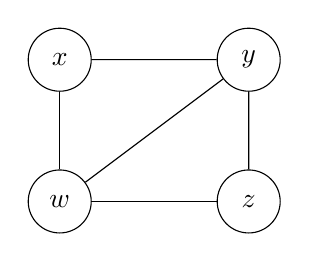
\begin{tikzpicture}[scale=1.2, every node/.style={circle, draw, minimum size=8mm}]

\node (x) at (0,1.5) {$x$};
\node (y) at (2,1.5) {$y$};
\node (z) at (2,0) {$z$};
\node (w) at (0,0) {$w$};

\draw (x) -- (y);
\draw (y) -- (z);
\draw (y) -- (w);
\draw (x) -- (w);
\draw (z) -- (w);

\end{tikzpicture}
\end{center}

\textbf{b)}
\begin{center}
\renewcommand{\arraystretch}{1.5}
\begin{tabular}{|c|c|c|}
\hline
\textbf{Edge} & \textbf{Reduced domain} & \textbf{Edges added to queue} \\
\hline
$(x,y)$ & none & none \\
\hline
$(x,w)$ & $D_x : \{1,2,3\} \to \{1,2\}$ & $(y,x)$ \\
\hline
$(y,x)$ & none & none \\
\hline
$(y,z)$ & none & none \\
\hline
$(y,w)$ & none & none \\
\hline
$(z,y)$ & none & none \\
\hline
$(z,w)$ & none & none \\
\hline
$(w,x)$ & $D_w : \{1,2,3\} \to \{1,2\}$ & $(y,w), (z,w)$ \\
\hline
$(w,y)$ & none & none \\
\hline
$(w,z)$ & none & none \\
\hline
$(y,x)$ & none & none \\
\hline
$(y,w)$ & none & none \\
\hline
$(z,w)$ & none & none \\
\hline
\end{tabular}
\end{center}

\end{solution}



\question[25] 
Consider the MDP graph: states are nodes, and there is a directed edge of the form $(s,s')$ if there is some action $a$ such that $\Pr[\delta(s,a) = s'] > 0$. In other words, there is an edge from $s$ to $s'$ if some action leads from $s$ to $s'$ with positive probability. 
Note that under this definition, terminal states do not have any outgoing edges.

Suppose that the MDP graph is acyclic. Present an algorithm for computing the optimal policy for acyclic MDPs. What is the runtime of your algorithm? 

\begin{solution}


\noindent\textbf{1) Pseudocode:}

\begin{algorithmic}[1]
\State Topologically sort the MDP graph.
\For{every state $s$}
    \State $V^*(s) \gets 0$
\EndFor
\Statex
\For{states $s$ in reverse topological order}
    \If{$A(s) = \emptyset$}
        \State $V^*(s) \gets 0$
    \Else
        \State
        \[
        V^*(s) \gets 
        \max_{a \in A(s)}
        \left[
        r(s,a) + \gamma \sum_{s'} \Pr(s' \mid s,a)V^*(s')
        \right]
        \]
        \State $\pi^*(s) \gets$ an action $a$ with max rewards
    \EndIf
\EndFor
\Statex
\State \Return $V^*$ and $\pi^*$
\end{algorithmic}

\textbf{2) Running Time:}
\[\mathcal{O}(|S| + |E| + |A|) \qquad S:\ State,\ E:\ Edge,\ A:\ Action\]

\end{solution}


\question[35]
Tammy is training for a marathon, which takes place in three weeks. She needs to train for the marathon, however, she's recovering from an injury. Each week, she can either train or rest. 
\begin{itemize}
    \item If she trains while injured, she gets a reward of 1.
    \item If she trains while fully recovered, she gets a reward of 2.
    \item If she rests, she gets a reward of 0.
\end{itemize}
When Tammy trains while injured, she has a 50\% chance of being fully recovered the following week. If she decides to rest instead, this probability increases to 80\%. Suppose that once she recovers, she does not get injured again. Tammy does not earn any additional rewards after week 3, regardless of her being fully recovered or not. 
\begin{parts}
    \part[10] Describe this problem as an MDP. Describe the states, actions at each state, and transition model. Indicate which states are terminal nodes, and the reward function in each state. \\ \textbf{Hint:} When modeling the problem, it is useful to have states representing Tammy being recovered or not on each week (except for week 1, she cannot be recovered then), and one terminal state for the marathon itself. 
    \begin{solution}

\text{1) State:} \[S = \{I_1, I_2, R_2, I_3, R_3, T\}\]
\text{2) Action:} \[Non-Terminate:\{train, rest\}\]
\[Terminate: \{None\}\]
\text{3) Transition Model:}

\begin{itemize}
    \item \textbf{From injured states}
    \begin{itemize}
        \item Tammy + injured  + train:
        \[
        I_t \xrightarrow{\text{train}}
        \begin{cases}
        R_{t+1}, & 0.5,\\
        I_{t+1}, & 0.5.
        \end{cases}
        \]

        \item Tammy + injured + rest:
        \[
        I_t \xrightarrow{\text{rest}}
        \begin{cases}
        R_{t+1}, & 0.8,\\
        I_{t+1}, & 0.2.
        \end{cases}
        \]
    \end{itemize}

    \item \textbf{From recovered states}

    \begin{itemize}
        \[
        R_t \xrightarrow{\text{train}} R_{t+1}
        \]
        \[
        R_t \xrightarrow{\text{rest}} R_{t+1}
        \]
    \end{itemize}

    \item \textbf{Week 3 transitions}

    \begin{itemize}
        \[
        I_3 \xrightarrow{\text{train}} T
        \]
        \[
        I_3 \xrightarrow{\text{rest}} T
        \]
        \[
        R_3 \xrightarrow{\text{train}} T
        \]
        \[
        R_3 \xrightarrow{\text{rest}} T
        \]
    \end{itemize}
\end{itemize}

\textbf{4) Reward Model:}
\[
r(I_1,train) = r(I_2,train) = r(I_3,train) = 1
\]
\[
r(R_2,train) = r(R_3,train) = 2
\]
\[
r(rest) = 0
\]
    
    \end{solution}
    
    \part[5] What are the possible (deterministic) policies are there for this MDP?
    \begin{solution}
\[2^{5} = 32\]

    \end{solution}

    \part[10] Suppose Tammy decides to train every week. What is Tammy's value at every state for this policy as a function of the discount factor $\gamma$?
    \begin{solution}
\[
V^\pi(T) = 0
\]
\[
V^\pi(I_3) = 1, \qquad V^\pi(R_3) = 2
\]
\[
V^\pi(I_2) = 1 + 1.5\gamma, \qquad V^\pi(R_2) = 2 + 2\gamma
\]
\[
V^\pi(I_1) = 1 + 1.5\gamma + 1.75\gamma^2
\]
    
    \end{solution}

    \part[10] Compare the reward of the policy of training every week, to the policy of resting on the first week, and then training on weeks 2 and 3. For what values of the discount factor $\gamma$ is one policy better than the other?
    \begin{solution}
\[
V_A(I_1)=1+1.5\gamma+1.75\gamma^2
\]
\[
V_B(I_1)=1.8\gamma+1.9\gamma^2
\]
1) Compare:
\[
1+1.5\gamma+1.75\gamma^2
>
1.8\gamma+1.9\gamma^2
\]
\[
1-0.3\gamma-0.15\gamma^2>0
\]
\[
1-0.3\gamma-0.15\gamma^2=0
\]
\[
20-6\gamma-3\gamma^2=0
\]
\[
3\gamma^2+6\gamma-20=0
\]
\[
\gamma=\frac{-6\pm\sqrt{36+240}}{6} = \frac{-6\pm\sqrt{276}}{6} = \frac{-3\pm\sqrt{69}}{3} =\frac{-3+\sqrt{69}}{3}
\]
\[
\frac{-3+\sqrt{69}}{3}\approx 1.77
\]
\[
V_A(I_1)>V_B(I_1),\quad  0\le\gamma\le1 < 1.77
\]
    \end{solution}
\end{parts}


\question[10] Consider the following modification of the greedy algorithm for learning a regret-minimizing policy in the expert systems domain.
Instead of picking an action out of the set of best-performing actions so far (as is the case for the simple greedy algorithm), we pick the best performing action in the previous $k$ time-steps; if there is more than one $k$-best performing action, we pick the one with the lowest index. For example, if $k = 1$, we simply pick any one of the actions that offered the highest reward in the previous round; if $k = 3$, we pick the action that had the highest cumulative reward in the last three rounds, etc.
More formally, the $k$-greedy algorithm works as follows. At time $t$, let $S_t$ be the set of actions that had maximal total reward at time steps $t - k, . . . , t - 1$; we pick the action with the lowest index out of $S_t$ (if $t \le k$ we run the original greedy algorithm).
What is the worst-case regret of the $k$-greedy algorithm? You must provide a formal proof of its regret guarantees with respect to the best action.
\begin{solution}
\[
R_T = V_{\mathrm{best}}(T)-V_{\mathrm{alg}}(T),
\qquad V_{\mathrm{best}}(T)=\max_i \sum_{t=1}^T r_t(i),
\qquad
V_{\mathrm{alg}}(T)=\sum_{t=1}^T r_t(A_t).
\]
Assume rewards are in \(\{0,1\}\).

\text{1) Upper Bound:}
\[
R_T \le T,
\]

2) Lower Bound, let's consider two actions \(a_1,a_2\). 
\[
r_t(A_t)=0, \qquad A_t \text{ is the action alg choose}
\]
\[
r_t(a)=1. \qquad a \neq A_t
\]

Then
\[
V_{\mathrm{alg}}(T)=\sum_{t=1}^T r_t(A_t)=0.
\]

Also, in every round,
\[
r_t(a_1)+r_t(a_2)=1.
\]
Hence
\[
\sum_{t=1}^T r_t(a_1)+\sum_{t=1}^T r_t(a_2)=T.
\]
Therefore,
\[
V_{\mathrm{best}}(T)
=
\max\left\{
\sum_{t=1}^T r_t(a_1),
\sum_{t=1}^T r_t(a_2)
\right\}
\ge \frac{T}{2}.
\]

Thus,
\[
R_T
=
V_{\mathrm{best}}(T)-V_{\mathrm{alg}}(T)
\ge
\frac{T}{2}-0
=
\frac{T}{2}.
\]

\[
R_T=\Theta(T)
\]

\end{solution}
\question[bonus]
Consider the no regret learning setting we have studied in class. We saw that in order to achieve a low regret, we need a sufficiently large number of rounds. 
What happens when the number of rounds is small? Prove that if there are $n$ experts and $T$ time steps, such that $T < \lfloor\log_2 n\rfloor$, then for any randomized algorithm $\cal A$, there is some randomized assignment of losses\footnote{Here we consider losses instead of rewards, but the idea is similar.} in $\{0,1\}$ to the experts (which can depend on what $\cal A$ does) such that 
\begin{enumerate}
	\item 
	$\cal A$ incurs a loss of at least $\frac T2$.
	\item 
	There exists at least one action that has a loss of 0.
\end{enumerate}
You may assume (with not much loss of generality) that $n = 2^k$ for some positive integer $k$.
\begin{solution}
\[
n=2^k,\qquad T<\lfloor \log_2 n\rfloor
\]
\[
S_0=\{1,2,\dots,n\}
\]

\text{1)}

At round \(t\), let \(p_t(i)\) be the probability that algorithm \(A\) chooses expert \(i\).

Split \(S_{t-1}\) into two equal parts:
\[
|S_t^0|=|S_t^1|=\frac{|S_{t-1}|}{2}.
\]

Define
\[
P_0=\sum_{i\in S_t^0}p_t(i),
\qquad
P_1=\sum_{i\in S_t^1}p_t(i).
\]

The adversary assigns loss \(1\) to the half with larger probability, and loss \(0\) to the other half.

Thus,
\[
\mathbb{E}[\ell_t(A)]
\ge
\max(P_0,P_1)
\ge
\frac{1}{2}.
\]

Therefore,
\[
\mathbb{E}[L_A]
=
\sum_{t=1}^T \mathbb{E}[\ell_t(A)]
\ge
\sum_{t=1}^T \frac{1}{2}
=
\frac{T}{2}.
\]

\text{2)}

After \(T\) rounds,

\[
|S_T|
=
\frac{n}{2^T}
=
\frac{2^k}{2^T}
=
2^{k-T}.
\]

Since \(T<k\),

\[
|S_T|=2^{k-T}\ge 1.
\]

Hence, there exists an expert \(i\in S_T\) such that
\[
L_i=0.
\]

\end{solution}

\end{questions}

\end{document}
















